\section{Changes to the Bifurcation Structure}
\label{sec:add.change}

\begin{enumerate}
	\item \begin{itemize}
		      \item ``type A'' parameter regions stop overlapping with the ``type A'' period regions above them (lower period, same number of points on branches $f_\B$ and $f_\D$)
		      \item Point where boundaries cross. On the left: no overlap, period-adding. On the right: overlap
		      \item This point moves right until no overlap exists anymore
	      \end{itemize}
	\item \begin{itemize}
		      \item ``type A'' parameter regions start overlapping with the ``type A'' period regions above right them (same period)
		      \item Point where boundaries cross. On the left: overlap. On the right: no overlap, ``type B'' parameter region
		      \item This point moves right, until no ``type B'' parameter region exists anymore
	      \end{itemize}
	\item \begin{itemize}
		      \item ``type A'' parameter regions stop overlapping with the ``type A'' parameter regions right to them (higher period, one more point on branches $f_\B$ and $f_\D$)
		      \item This seems to happen in an instant
	      \end{itemize}
\end{enumerate}

Timeline:
On the parameter line outlined above, the processes happen as follows.
First, the process (i) starts.
While it is happening, the process (ii) starts and finishes, before (i) finishes.
Lastly the process (iii) starts and finishes directly.
After all that, process (i) is the last to complete.

\todo{Remove previous}

\Cref{fig:add.change.regions} shows diagrams depicting the borders of parameter regions with different symbolic sequences.
We will use these diagrams as basis for our exploration of the changes to the bifurcation structure.
The lower left corner of the diagrams is always in the period region with the stable cycle $\Cycle{\A^7\B^3\C^7\D^3}$.
The cycles in the upper left ($\Cycle{\A^6\B^3\C^6\D^3}$), upper right ($\Cycle{\A^6\B^4\C^6\D^4}$), lower right ($\Cycle{\A^7\B^4\C^7\D^4}$), and middle ($\Cycle{\A^7\B^3\C^6\D^4}$ and $\Cycle{\A^6\B^4\C^7\D^3}$) follow.
We introduce a short notation for the symbolic sequences here.
``Type A'' parameter regions where the cycle is associated with the symbolic sequence $\A^a\B^b\C^a\D^b$ are written as $P^{2 \cdot \left(a + b\right)}_b$
``Type B'' parameter regions where the coexisting twin cycles are associated with the symbolic sequences $\A^a\B^b\C^c\D^d$ and $\A^c\B^d\C^a\D^b$ where $c = a - 1$ and $d = b + 1$ are written as $P^{a + b + c + d}_b$.
So for example, the ``type A'' parameter region in the lower left corner of every diagram in \Cref{fig:add.change.regions} is written as $P^{20}_3$.
\todo{
	Special case $\left[P^{2 \cdot \left(a + b\right)}_b \mid P^{2 \cdot \left(c + d\right)}_d\right]$ where $c \neq a - 1$ or $d \neq b + 1$ (it's not a ``type B'' parameter regions as we described them earlier).
	Where $c < a$ or $d > b$.
	Operation defined later in \Cref{sec:add.add.halved}.
}

The four different diagrams in \Cref{fig:add.change.regions} show the evolution at different points during the transition from \Cref{fig:add.arch} to \Cref{fig:add.arch.new}.
For this, the parameter values for $a_L$ and $b_L$ are chosen along a line given by \Cref{equ:add.change.paramline}
\begin{align}
	a_L = \frac{5}{2} - 3 \cdot b_L
	\label{equ:add.change.paramline}
\end{align}

\todo{Labels and remember to check parameters in captions / move to large caption}
\begin{figure}
	\centering
	\subfloat[$a_L = 2.8, b_L = -0.1$]{
		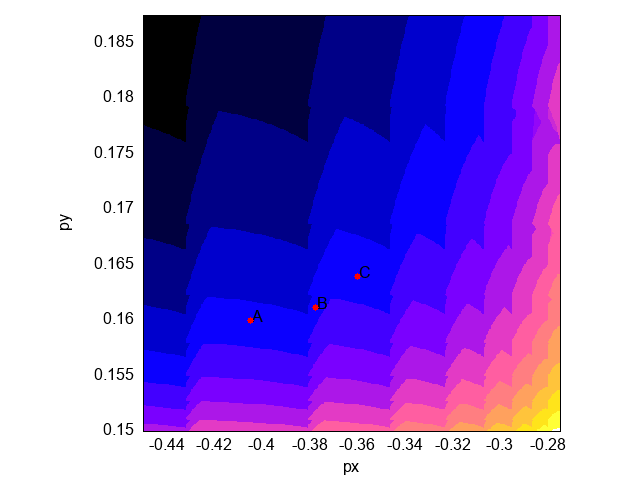
\includegraphics[width=.5 \textwidth]{62_MinimalRepr_Adding/2D_Regions_3.5/result-simple.png}
		\label{fig:add.change.regions.1}
	}
	\subfloat[$a_L = 2.8, b_L = -0.1$]{
		\includegraphics[width=.5 \textwidth]{62_MinimalRepr_Adding/2D_Regions_2.8/Manual/result.png}
		\label{fig:add.change.regions.2}
	} \\
	\subfloat[$a_L = 2.725, b_L = -0.075$]{
		\includegraphics[width=.5 \textwidth]{62_MinimalRepr_Adding/2D_Regions_2.725/Manual/result.png}
		\label{fig:add.change.regions.3}
	}
	\subfloat[$a_L = 2.65, b_L = -0.05$]{
		\includegraphics[width=.5 \textwidth]{62_MinimalRepr_Adding/2D_Regions_2.5/Manual/result.png}
		\label{fig:add.change.regions.4}
	}
	\caption{Evolution of ``type B'' parameter regions when transitioning to a period adding scenario}
	\label{fig:add.change.regions}
\end{figure}

First, we will examine the disappearance of the ``type B'' parameter regions.
After that, we will examine the appearance of period-adding structures between the chains of the same period.

\subsection{Disappearance of ``Type B'' Parameter Regions}
\label{sec.change.disb}

For \Cref{fig:add.change.regions.1,fig:add.change.regions.2}, the ``type B'' parameter region $Q^{20}_3$ is complete.
In \Cref{fig:add.change.regions.4}, it is gone completely, instead the two ``type A'' parameter regions $P^{20}_3$ and $P^{20}_4$ now overlap.
\todo{In regions figure 3: labels $P^{20}_2$ wrong, should be $P^{20}_4$}

In between those two stages, we can see how the ``type B'' parameter region $Q^{20}_3$ disappears.
\Cref{fig:add.change.regions.3} shows the ``type A'' parameter regions $P^{20}_3$ and $P^{20}_4$ overlapping.
The point, where their boundaries cross is in the middle of where the ``type B'' parameter region was in \Cref{fig:add.change.regions.2}.
This point is also where the ``type B'' parameter region now ends.

\todo{Labels in figure wrong!}
\todo{In cobweb diagrams: enhance cycles at borders}
\begin{figure}
	\centering
	\subfloat[Regions]{
		\includegraphics[width=.3 \textwidth]{62_MinimalRepr_Adding/2D_Regions_2.675/Manual/result.png}
		\label{fig:add.change.disb.regions}
	}
	\subfloat[Cobweb at point $A$]{
		\includegraphics[width=.3 \textwidth]{62_MinimalRepr_Adding/Cob_2.675_A/Manual/result.png}
		\label{fig:add.change.disb.cob.A}
	}
	\subfloat[Cobweb at point $B$]{
		\includegraphics[width=.3 \textwidth]{62_MinimalRepr_Adding/Cob_2.675_B/Manual/result.png}
		\label{fig:add.change.disb.cob.B}
	}
	\caption{Disappearance of the ``type B'' parameter region}
\end{figure}

\Cref{fig:add.change.disb.regions} shows the same thing as \Cref{fig:add.change.regions.3} again but at parameter value closer to the diappearence of the ``type B'' parameter region.
We can see that the point where the boundaries of the ``type A'' parameter regions cross moved right and the ``type B'' parameter region got smaller.
This point is called a codimension-2 point because at this point, two bifurcations happen at the same time to the same cycle.

We know from \Cref{sec:arch.bif.sum} that the \gls{bcb} at the upper boundary of the ``type A'' parameter region $P^{20}_3$ is $\BCB_{d_1, d_3}^{\underline{\A}^7\B^3\underline{\C}^7\D^3}$.
And the \gls{bcb} at the lower boundary of the ``type A'' parameter region $P^{20}_4$ is $\BCB_{d_1, d_3}^{\A^6\underline{\B}^4\C^6\underline{\D}^4}$.
At the codimension-2 point, both these \glspl{bcb} happen at the same time and both cycles vanish.
We can see in \Cref{fig:add.change.disb.cob.A} that the ``type A'' cycles are very close to the borders $d_1$ and $d_3$, respectively.

We also know that the \glspl{bcb} at the top of the ``type B'' parameter region $Q^{20}_3$ are $\BCB_{d_1}^{\underline{\A}^7\B^3\C^6\D^4}$ and $\BCB_{d_3}^{\A^6\B^4\underline{\C}^7\D^3}$.
And the \glspl{bcb} at the lower boundary are $\BCB_{d_3}^{\A^7\B^3\C^6\underline{\D}^4}$ and $\BCB_{d_1}^{\A^7\underline{\B}^3\C^6\D^4}$.
At the codimension-2 point, both \glspl{bcb} $\BCB_{d_1}^{\underline{\A}^7\B^3\C^6\D^4}$ and $\BCB_{d_3}^{\A^7\B^3\C^6\underline{\D}^4}$ happen to the cycle $\Cycle{\A^7\B^3\C^6\D^4}$ at the same time and it vanishes.
Because of the symmetry, the \glspl{bcb} $\BCB_{d_3}^{\A^6\B^4\underline{\C}^7\D^3}$ and $\BCB_{d_1}^{\A^7\underline{\B}^3\C^6\D^4}$ happen to the cycle $\Cycle{\A^6\B^4\C^7\D^3}$ at the same time and it vanishes also.

This codimension-2 point moves right with higher values for $b_L$ along our line.
As soon as the codimension-2 point crosses the right boundary of the ``type B'' parameter region, the ``type B'' parameter region ceases to exist.
Instead, now the two ``type A'' parameter regions overlap without the codimension-2 point.
This new overlapping regions is bounded by simple ``type A'' boundary \glspl{bcb} as they are discussed in \Cref{sec:arch.bif.sum}.

\todo{Confirm bcbs with cobweb diagrams}

\todo{Order of left most cycle and other cycle => type B or type A. idk}

\subsection{Appearance of Period-adding structures}

In this section we will explore the appearance of the period-adding structures in between the chains of the same period.
This happens at the horizontal boundaries between ``type A'' parameter regions of different chains, as well as at the vertical boundaries.
We will first take care of the horizontal period-adding structures and then move on to the vertical period-adding structures.

\subsubsection{Horizontal Period-adding Structures}

In \Cref{fig:add.change.regions.1}, the ``type A'' parameter regions $P^{20}_3$ and $P^{18}_3$, as well as $P_{22}_4$ and $P^{20}_4$ overlap.
This changes in \Cref{fig:add.change.regions.2}.
Here only the ``type A'' parameter regions $P^{20}_3$ and $P^{18}_3$ overlap, the parameter regions $P_{22}_4$ and $P^{20}_4$ stopped overlapping.
Instead, in the space between the two ``type A'' parameter region there are now two asymmetric coexisting twin cycles $\Cycle{\A^8\B^3\C^8\D^2}$ and $\Cycle{\A^8\B^2\C^8\D^3}$.
Those cycles are \textbf{not} ``type B'' cycles, because they only differ in the number of points on the branches $f_\B$ and $f_\D$.
Instead, we will call them hybrid cycles and ``type B'' cycles are a special case of hybrid cycles.
The notation $\left[P^{22}_4 \mid P^{20}_4\right]$ used in the diagrams was introduced in \Cref{sec:add.change} and is formally defined later in \Cref{sec:add.add.halved}.
Later in \Cref{fig:add.change.regions.4}, the ``type A'' parameter regions $P^{20}_3$ and $P^{18}_3$ also stop overlapping.
In between, there are also hybrid cycles, $\Cycle{\A^7\B^3\C^6\D^3}$ and $\Cycle{\A^6\B^3\C^7\D^3}$.
This parameter region is therefore labeled $\left[P^{20}_3 \mid P^{18}_3\right]$.

In between \Cref{fig:add.change.regions.2,fig:add.change.regions.3}, the ``type A'' parameter regions $P_{22}_4$ and $P^{20}_4$ don't stop overlapping completely.
Instead, they only stop overlapping on the left side of their shared boundaries and the rest is not pictured in these diagrams.
\Cref{fig:add.change.appa.hor.regions} shows better what happens to this overlapping region between \Cref{fig:add.change.regions.1,fig:add.change.regions.4}.
We also have a codimension-2 point that moves right as was the case in \Cref{sec:add.change.disb}.

\todo{Regions: labels wrong}
\todo{Cobwebs: enhance borders, replace (c), wrong pic}
\begin{figure}
	\centering
	\subfloat[Regions]{
		\includegraphics[width=.3 \textwidth]{62_MinimalRepr_Adding/2D_Regions_2.8_add_hor/Manual/result.png}
		\label{fig:add.change.appa.hor.regions}
	}
	\subfloat[At point $A$]{
		\includegraphics[width=.3 \textwidth]{62_MinimalRepr_Adding/Cob_2.8_add_hor_A/Manual/result.png}
		\label{fig:add.change.appa.hor.cob.A}
	}
	\subfloat[At point $B$]{
		\includegraphics[width=.3 \textwidth]{62_MinimalRepr_Adding/Cob_2.8_add_hor_A/Manual/result.png}
		\label{fig:add.change.appa.hor.cob.B}
	}
	\caption{Appearance of the horizontal period-adding cascade}
\end{figure}

We know from \Cref{sec:arch.bif.sum} that the \gls{bcb} at the upper boundary of the ``type A'' parameter region $P^{22}_4$ is $\BCB_{d_1, d_3}^{\underline{\A}^7\B^4\underline{\C}^7\D^4}$.
And the \gls{bcb} at the lower boundary of the ``type A'' parameter region $P^{20}_4$ is $\BCB_{d_1, d_3}^{\A^6\underline{\B}^4\C^6\underline{\D}^4}$.
Both these \glspl{bcb} are at the upper and lower boundaries of the overlapping region $P^{22}_4 \Cup P^{20}_4$.
At the codimension-2 point, both these \glspl{bcb} happen at the same time and both cycles vanish.
We can see in \Cref{fig:add.change.appa.hor.cob.A} that the ``type A'' cycles are very close to the borders $d_1$ and $d_3$, respectively.

This codimension-2 point moves right with higher values for $b_L$ along our line.
As soon as the codimension-2 point crosses the right boundary of either the ``type A'' parameter region $P^{22}_4$ or $P^{20}_4$, the overlapping parameter region $P^{22}_4 \Cup P^{20}_4$ ceases to exist.
Instead, there is space between the two ``type A'' parameter regions where the are now two hybrid cycles and period-adding between the hybrid cycles and either ``type A'' parameter region.

\todo{Labels for bifurcations missing underline}
\begin{figure}
	\centering
	\includegraphics[width=.7 \textwidth]{62_MinimalRepr_Adding/1D_Bif_2.8_add_hor_AU/Manual/result.png}
	\caption{Bifurcation diagram at the upper boundary of $\left[P^{22}_4 \mid P^{20}_4\right]$}
	\label{fig:add.change.appa.hor.bif}
\end{figure}

We assume that the \glspl{bcb} bounding the parameter regions with hybrid cycles follow the same rules as the \glspl{bcb} bounding the ``type B'' parameter regions.
\Cref{fig:add.change.appa.hor.bif} confirms this for the upper boundary.
So it is bounded at the top by the \glspl{bcb} $\BCB_{d_1}^{\underline{\A}^7\B^4\C^6\D^4}$ and $\BCB_{d_3}^{\A^6\B^4\underline{\C}^7\D^4}$.
And bounded at the bottom by the \glspl{bcb} $\BCB_{d_3}^{\A^7\B^4\C^6\underline{\D}^4}$ and $\BCB_{d_1}^{\underline{\A}^6\B^4\C^7\D^4}$.
At the codimension-2 point, both \glspl{bcb} $\BCB_{d_1}^{\underline{\A}^7\B^4\C^6\D^4}$ and $\BCB_{d_3}^{\A^7\B^4\C^6\underline{\D}^4}$ happen to the cycle $\Cycle{\A^7\B^4\C^6\D^4}$ at the same time and it vanishes.
Because of the symmetry, the \glspl{bcb} $\BCB_{d_3}^{\A^6\B^4\underline{\C}^7\D^4}$ and $\BCB_{d_1}^{\A^6\underline{\B}^4\C^7\D^4}$ happen to the cycle $\Cycle{\A^6\B^4\C^7\D^4}$ at the same time and it vanishes also.

\todo{also confirmed by cobweb with enhanced cycles at borders}

\todo{Parallels to disappearing type B}

\todo{old:}

In \Cref{sec:minrep.adding.disapp.typeB}, we noted that the asymmetry of the ``type B'' cycles is caused by the negative slope of the function at the left border of branches $f_\A$ and $f_\C$.
Since this maps the cycle that starts further left to the right side of the other cycle.
\todo{
	explain better: diff number of points on branches B and D each (type B) therefore reordering necessary for asymm.
	type b also: split at $d_1, d_3$ as well as $d_2$ and $d_0$, here only $d_1, d_3$ (two boundaries).
	here same number of points so there must be no reordering for asymm
}
This is not the case for the cycles at this point, both cycles start at a point on the branch $f_\A$ with a positive slope and therefore keep the same order.
\todo{positive slope important for period adding!}

\subsubsection{Vertical}

\todo{Regions: labels wrong}
\todo{Cobwebs: replace (c) and enhance cycles at borders}
\begin{figure}
	\centering
	\subfloat[Regions scan before period-adding\\at $a_L = 2.8, b_L = -0.1$]{
		\includegraphics[width=.4 \textwidth]{62_MinimalRepr_Adding/2D_Regions_2.8_add_vert/Manual/result.png}
		\label{fig:minrep.add.app.vert.reg.before}
	}
	\subfloat[Regions with period-adding\\at $a_L = 2.65, b_L = -0.05$]{
		\includegraphics[width=.4 \textwidth]{62_MinimalRepr_Adding/2D_Regions_2.65_add_vert/Manual/result.png}
		\label{fig:minrep.add.app.vert.reg.with}
	} \\
	\subfloat[At point $A$]{
		\includegraphics[width=.4 \textwidth]{62_MinimalRepr_Adding/Cob_2.8_add_vert_A/Manual/result.png}
		\label{fig:minrep.add.app.vert.cob.A}
	}
	\subfloat[At point $B$]{
		\includegraphics[width=.4 \textwidth]{62_MinimalRepr_Adding/Cob_2.65_add_vert_B/Manual/result.png}
		\label{fig:minrep.add.app.vert.cob.B}
	}
	\caption{Appearance of the vertical period-adding cascade}
	\label{fig:minrep.add.app.vert}
\end{figure}

For the vertical period-adding cascade, it is similar.
This time one parameter region scan is not enough because the boundaries of $P_{10}^3$ and $P_{11}^4$ are parallel and therefor $P_{10}^3 \bigcup P_{11}^4$ and $P_{10}^3 \oplus P_{11}^4$ can't exist at the same parameter values of $a_L$ and $b_L$.
\Cref{fig:minrep.add.app.vert.reg.before} shows the situation before the vertical period-adding cascade appears.
Here we can see the overlap of the two ``type A'' parameter regions $P_{10}^3$ and $P_{11}^4$.
When changing the parameters a little, we get \Cref{fig:minrep.add.app.vert.reg.with}.
Here the two ``type A'' parameter regions drifted apart and in between them, there is the parameter region $P_{10}^3 \oplus P_{11}^4$.
The notation hints at the period-adding-like nature of this parameter region.

As with the horizontal period-adding cascade, the cycles here are asymmetrical, but not of ``type B''.
\Cref{fig:minrep.add.app.vert.cob.B} shows the cycles at point $B$, in the period adding cascade, $\Cycle{\A^7\B^3\C^7\D^4}$ and its twin $\Cycle{\A^7\B^4\C^7\D^3}$.
Again, interpreted in the context of the halved model, these cycles are both $\Cycle{\L^7\R^3\L^7\R^4} \equiv \Cycle{\L^7\R^4\L^7\R^3}$.
But this time, the splits are not at borders $d_1$ and $d_3$, but at $d_0$ and $d_2$.
\todo{odd number of splits => no neg slope needed for asymmetry. odd number => needed (reorders cycles)}

\begin{figure}
	\centering
	\includegraphics[width=.7 \textwidth]{62_MinimalRepr_Adding/1D_Bif_2.65_add_vert_BR/Manual/result.png}
	\caption{Bifurcation diagram of the right boundary of $P_{10}^3 \oplus P_{11}^4$}
	\label{fig:minrep.add.app.vert.bif.BR}
\end{figure}

Here, the period-adding region opened up enough to see the next stage, colored in purple.
As with the previous bifurcations of the first stage of the horizontal period-adding cascade, the bifurcations are similar to the bifurcations of ``type B'' cycles in \Cref{sec:minrep.bif.R}.
They involve the borders $d_0$ and $d_2$.
\todo{etc}

